% ====================================================================
% BAB 3: METODOLOGI PENELITIAN
% ====================================================================
% File ini berisi metodologi penelitian yang mencakup:
% - Lokasi dan waktu penelitian
% - Populasi dan sampel
% - Data penelitian (jenis dan sumber)
% - Prosedur penelitian
% - Metode analisis
%
% EDIT konten sesuai dengan metodologi penelitian Anda.
% ====================================================================

\chapter{METODOLOGI PENELITIAN}

% --- BAGIAN 3.1: LOKASI DAN WAKTU PENELITIAN ---
\section{Jenis Penelitian}
\label{sec:method-type}

Penelitian ini termasuk kategori kuantitatif eksperimental dengan pendekatan Research and Development (R\&D).
Aspek R\&D terletak pada pengembangan sistem analisis topik percakapan WhatsApp berbasis web,
sedangkan aspek eksperimental kuantitatif digunakan untuk memvalidasi performa pipeline BERTopic dengan modifikasi IndoBERTweet sebagai model embedding dan BIRCH sebagai model clustering yang diimplementasikan dalam sistem.

% --- BAGIAN 3.2: POPULASI DAN SAMPEL ---
\section{Objek Penelitian}
\label{sec:method-object}

Objek penelitian fokus pada data percakapan grup WhatsApp yang berisi
interaksi antar pengguna dalam bahasa Indonesia. Data ini dipilih karena
mewakili karakteristik percakapan yang umumnya berupa teks pendek, tidak
terstruktur, mengandung \textit{noise}, serta fenomena \textit{code-mixing}.
Karakteristik tersebut menjadikan data percakapan grup WhatsApp relevan untuk
menguji kemampuan pipeline BERTopic yang dimodifikasi dalam menghasilkan topik
yang koheren dan stabil.

\section{Waktu Penelitian}
\label{sec:time}

Waktu penelitian dilakukan pada bulan April 2026 hingga Juni 2026, dengan tahapan-tahapan yang telah direncanakan secara sistematis untuk memastikan kelancaran proses penelitian.

\section{Tahapan Penelitian}
\label{sec:stages}

Tahapan penelitian yang dilakukan dalam penelitian ini secara keseluruhan
digambarkan pada \textbf{Gambar \ref{fig:tahapan-penelitian}}:

\begin{figure}[H]
	\centering
	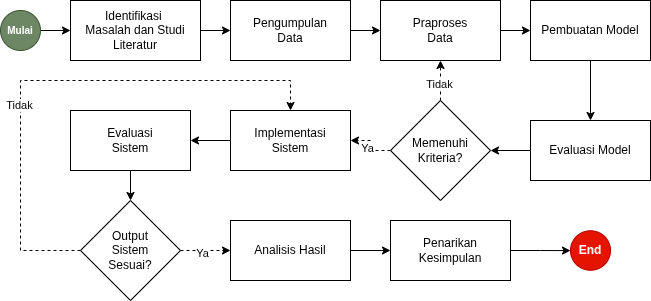
\includegraphics[width=0.85\textwidth]{images/alur_penelitian.png}
	\caption{Tahapan Penelitian}
	\label{fig:tahapan-penelitian}
\end{figure}

\subsection{Identifikasi Masalah dan Studi Literatur}
\label{subsec:problem-identification}

Tahap pertama dalam penelitian ini adalah identifikasi masalah dan studi
literatur. Peneliti melakukan eksplorasi awal terhadap fenomena percakapan grup
WhatsApp untuk memahami tantangan dalam menangkap topik pembicaraan secara
menyeluruh, mencakup dinamika percakapan, karakteristik teks, serta kebutuhan
pengguna dalam mengelola informasi yang besar dan tidak terstruktur.

Studi literatur kemudian dilakukan untuk membangun landasan teori dan memahami
perkembangan terkini di bidang \textit{topic modeling} berbahasa Indonesia melalui
kajian jurnal ilmiah, prosiding konferensi, dan dokumentasi teknis terkait BERTopic,
IndoBERTweet, BIRCH \textit{clustering}, BM25, serta metrik evaluasi pemodelan topik.
Hasil gabungan tahap ini digunakan untuk mengidentifikasi \textit{research gap},
merumuskan masalah penelitian secara spesifik, dan menentukan metode serta
arsitektur sistem yang akan dikembangkan.

\subsection{Pengumpulan Data}
\label{subsec:data-collection}

Tahap pengumpulan data dilakukan dengan mengekspor riwayat percakapan dari grup
WhatsApp menggunakan fitur \textit{export chat} yang tersedia secara bawaan pada
aplikasi WhatsApp. Data yang diekspor berupa file teks (\textit{.txt}) atau format \textit{.zip} yang memuat
informasi tanggal, waktu, nama pengirim, dan isi pesan. Data percakapan yang
dikumpulkan hanya bersumber dari satu grup WhatsApp, dengan rentang waktu maksimal
satu tahun data terbaru untuk memastikan relevansi topik dan menjaga fokus analisis
pada dinamika percakapan yang aktual.

\subsection{Praproses Data}
\label{subsec:data-preprocessing}

Tahap pra-pemrosesan data dibagi menjadi dua tahap, yaitu sebelum
\textit{embedding} model dan sebelum representasi topik.

\noindent \textbf{Tahap 1: Pra-\textit{Embedding} Model}

\noindent Tahap ini bertujuan membersihkan dan mempersiapkan data mentah agar siap diolah
oleh model \textit{embedding} dengan tetap mempertahankan makna semantik. Prosesnya meliputi:
\begin{enumerate}[nosep]
	\item Pemfilteran pesan sistem, yaitu menghapus notifikasi bawaan
	      WhatsApp seperti pesan bergabung, keluar grup, perubahan keamanan,
	      serta pesan media yang tidak disertakan.
	\item Konversi teks menjadi huruf kecil (\textit{lower-case}).
	\item Normalisasi \textit{mention} dan URL, dengan mengganti
	      nama pengguna menjadi \textit{@USER} dan URL menjadi \textit{HTTP}.
	\item Transliterasi emotikon.
	\item Normalisasi kata slang dan pemanjangan kata.
\end{enumerate}

\noindent \textbf{Tahap 2: Pra-Representasi Topik}

\noindent Tahap ini dilakukan sebelum pembentukan representasi topik, yaitu dengan
konfigurasi \textit{vectorizer} menggunakan \textit{stopword} dari kamus manual
dan \textit{library} Sastrawi.

\subsection{Pembuatan Model}
\label{subsec:create-model}

Tahap pemodelan topik merupakan tahap inti dari penelitian ini, di mana data
yang telah melalui pra-pemrosesan dianalisis menggunakan \textit{framework} BERTopic
yang telah dimodifikasi. Penentuan parameter pada tiap komponen dilakukan dengan
dua skenario, yaitu mengacu pada \textit{baseline} dari penelitian terdahulu dan
eksperimen penalaan parameter untuk memperoleh kinerja terbaik berdasarkan metrik
evaluasi. Alur pembuatan model ini terdiri dari empat komponen utama:

\begin{figure}[H]
	\centering
	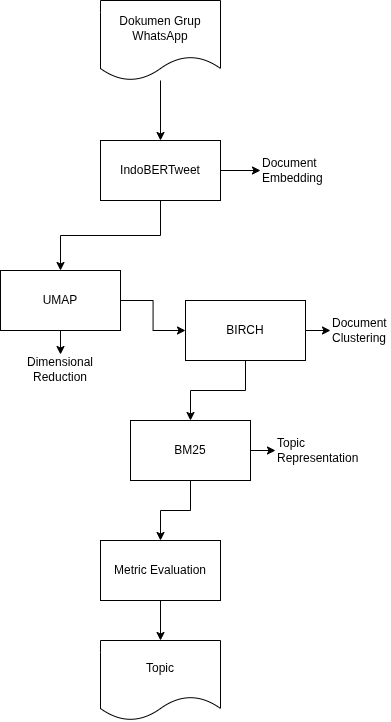
\includegraphics[width=0.5\textwidth]{images/framework-BERTopic-modifikasi.png}
	\caption{Rancangan framework BERTopic yang dimodifikasi pada tahap pembuatan model}\label{fig:framework-bertopic-modifikasi}
\end{figure}

\begin{enumerate}[nosep]
	\item \textbf{\textit{Document Embedding} menggunakan IndoBERTweet} \\
	      Setiap dokumen (pesan) diubah menjadi representasi vektor numerik
	      berdimensi tinggi menggunakan model IndoBERTweet yang telah diadaptasi
	      untuk teks media sosial berbahasa Indonesia. Representasi \textit{embedding} ini
	      mampu menangkap makna semantik dan konteks kata secara lebih akurat
	      dibandingkan model \textit{multilingual} \citep{koto2021indobertweet}.

	\item \textbf{\textit{Dimensionality Reduction} menggunakan UMAP} \\
	      Vektor \textit{embedding} berdimensi tinggi direduksi menggunakan
	      \textit{Uniform Manifold Approximation and Projection} (UMAP) untuk
	      mengurangi kompleksitas komputasi sambil mempertahankan struktur lokal
	      dan global data dalam ruang berdimensi rendah. Parameter UMAP yang
	      digunakan meliputi \textit{n\_neighbors}, \textit{n\_components},
	      \textit{min\_dist}, dan \textit{metric}.

	\item \textbf{\textit{Clustering} menggunakan BIRCH} \\
	      Dokumen yang telah direduksi dimensinya dikelompokkan menggunakan
	      algoritma BIRCH (\textit{Balanced Iterative Reducing and Clustering
		      using Hierarchies}) sebagai pengganti HDBSCAN standar. BIRCH dipilih
	      karena kemampuannya dalam mengalokasikan seluruh dokumen ke dalam
	      klaster tanpa menghasilkan \textit{outlier} dalam jumlah besar, serta
	      efisiensi komputasi dan penggunaan memori yang lebih baik. Parameter
	      BIRCH yang digunakan meliputi \textit{threshold},
	      \textit{branching\_factor}, dan \textit{n\_clusters}.

	\item \textbf{\textit{Topic Representation} menggunakan BM25} \\
	      Setiap klaster yang terbentuk direpresentasikan menggunakan skema
	      pembobotan BM25 sebagai pengganti c-TF-IDF bawaan BERTopic. BM25
	      menerapkan saturasi frekuensi istilah dan normalisasi panjang dokumen,
	      sehingga menghasilkan kata kunci representatif yang lebih relevan dan
	      stabil secara semantik untuk setiap topik. Parameter BM25 yang digunakan
	      meliputi \textit{k1} dan \textit{b}.
\end{enumerate}

\subsection{Evaluasi Model}
\label{subsec:model-evaluation}

Tahap evaluasi model bertujuan untuk mengukur kualitas topik yang dihasilkan
oleh model BERTopic secara kuantitatif. Evaluasi dilakukan menggunakan empat
metrik utama, yaitu:
\begin{enumerate}[nosep]
	\item \textit{Topic Coherence} (NPMI) untuk mengukur sejauh mana
	      kata-kata teratas dalam setiap topik memiliki hubungan semantik satu
	      sama lain. Nilai yang lebih tinggi menunjukkan topik yang lebih koheren.
	\item \textit{Topic Diversity} (TD) untuk mengukur keunikan kata-kata
	      teratas antar topik. Nilai mendekati 1 menunjukkan tidak ada tumpang
	      tindih kata antar topik.
	\item \textit{Embedding Density} untuk mengukur tingkat kekompakan
	      dokumen dalam tiap klaster pada ruang \textit{embedding}. Nilai yang
	      lebih tinggi menunjukkan klaster yang semakin padat.
	\item \textit{Intra-topic Similarity} untuk mengukur rata-rata
	      kesamaan semantik antar dokumen dalam satu topik. Nilai yang lebih
	      tinggi menunjukkan homogenitas topik yang lebih baik.
\end{enumerate}

\subsection{Implementasi Sistem}
\label{subsec:system-implementation}

Tahap pengembangan sistem bertujuan untuk mengimplementasikan seluruh alur
pemodelan topik ke dalam sebuah aplikasi berbasis web yang dapat digunakan
secara praktis oleh pengguna. Sistem ini memungkinkan pengguna untuk mengunggah
data ekspor percakapan grup WhatsApp, melakukan analisis topik secara otomatis,
serta menampilkan hasil pemodelan topik dalam bentuk visualisasi yang intuitif
dan informatif. Implementasi dilakukan dengan arsitektur \textit{client-server},
dengan Vue.js sebagai \textit{client} (antarmuka pengguna) dan FastAPI sebagai
\textit{server} (layanan API pemrosesan analisis topik). Pengembangan sistem
dilakukan menggunakan pendekatan terstruktur dengan memperhatikan aspek
fungsionalitas, kemudahan penggunaan (\textit{usability}), dan efisiensi
pemrosesan.

\subsection{Evaluasi Sistem}
\label{subsec:system-evaluation}

Tahap evaluasi sistem dilakukan untuk mengukur kinerja dan efektivitas aplikasi	yang telah dikembangkan. Evaluasi dilakukan dengan menggunakan metode black-box testing, di mana fokusnya adalah pada input dan output sistem tanpa memperhatikan proses internalnya. Pengujian dilakukan dengan menggunakan dataset percakapan grup WhatsApp yang berbeda dari dataset yang digunakan untuk pelatihan model, untuk memastikan bahwa sistem dapat bekerja secara umum dan tidak hanya pada data tertentu. Hasil evaluasi ini akan memberikan gambaran tentang seberapa baik sistem dapat mengidentifikasi dan merepresentasikan topik dalam percakapan grup WhatsApp secara otomatis, serta memberikan umpan balik untuk perbaikan lebih lanjut jika diperlukan.

\subsection{Analisis Hasil}
\label{subsec:result}

Tahap analisis hasil dilakukan terhadap seluruh keluaran dari pemodelan topik
dan evaluasi model. Analisis dilakukan dengan membandingkan performa model
berdasarkan metrik evaluasi yang telah ditentukan, serta menginterpretasikan
topik-topik yang dihasilkan.

\subsection{Penarikan Kesimpulan}

Berdasarkan hasil analisis, dilakukan penarikan kesimpulan yang menjawab
rumusan masalah penelitian serta penyusunan saran untuk pengembangan penelitian
di masa mendatang.

% ====================================================================
% CATATAN PENGISIAN BAB METODOLOGI:
%
% 1. LOKASI & WAKTU:
%    - Spesifik dan jelas (bukan abstrak)
%    - Jelaskan alasan pemilihan lokasi
%    - Sertakan durasi penelitian
%
% 2. POPULASI & SAMPEL:
%    - Definisikan populasi dengan jelas
%    - Jelaskan kriteria inklusi/eksklusi
%    - Tunjukkan perhitungan ukuran sampel
%    - Jelaskan metode sampling
%
% 3. DATA:
%    - Sebutkan jenis data (primer/sekunder, kualitatif/kuantitatif)
%    - Jelaskan sumber data spesifik
%    - Descripsikan instrumen pengumpulan data
%    - Sertakan validitas/reliabilitas instrumen
%
% 4. PROSEDUR:
%    - Urut kronologis dan logis
%    - Detail namun tidak berbelit-belit
%    - Jelaskan setiap tahap dengan jelas
%
% 5. ANALISIS:
%    - Jelaskan teknik analisis deskriptif
%    - Jelaskan uji statistik (jika ada) dengan detail
%    - Sertakan asumsi-asumsi uji
%    - Sebutkan software yang digunakan
% ====================================================================
